%% abtex2-modelo-relatorio-tecnico.tex, v-1.9.6 laurocesar
%% Copyright 2012-2016 by abnTeX2 group at http://www.abntex.net.br/ 
%%
%% This work may be distributed and/or modified under the
%% conditions of the LaTeX Project Public License, either version 1.3
%% of this license or (at your option) any later version.
%% The latest version of this license is in
%%   http://www.latex-project.org/lppl.txt
%% and version 1.3 or later is part of all distributions of LaTeX
%% version 2005/12/01 or later.
%%
%% This work has the LPPL maintenance status `maintained'.
%% 
%% The Current Maintainer of this work is the abnTeX2 team, led
%% by Lauro César Araujo. Further information are available on 
%% http://www.abntex.net.br/
%%
%% This work consists of the files abntex2-modelo-relatorio-tecnico.tex,
%% abntex2-modelo-include-comandos and abntex2-modelo-references.bib
%%

% ------------------------------------------------------------------------
% ------------------------------------------------------------------------
% abnTeX2: Modelo de Relatório Técnico/Acadêmico em conformidade com 
% ABNT NBR 10719:2015 Informação e documentação - Relatório técnico e/ou
% científico - Apresentação
% ------------------------------------------------------------------------ 
% ------------------------------------------------------------------------

\documentclass[
	% -- opções da classe memoir --
	12pt,				% tamanho da fonte
	openright,			% capítulos começam em pág ímpar (insere página vazia caso preciso)
	%twoside,			% para impressão em recto e verso. Oposto a oneside
	a4paper,			% tamanho do papel. 
	% -- opções da classe abntex2 --
	%chapter=TITLE,		% títulos de capítulos convertidos em letras maiúsculas
	%section=TITLE,		% títulos de seções convertidos em letras maiúsculas
	%subsection=TITLE,	% títulos de subseções convertidos em letras maiúsculas
	%subsubsection=TITLE,% títulos de subsubseções convertidos em letras maiúsculas
	% -- opções do pacote babel --
	english,			% idioma adicional para hifenização
	french,				% idioma adicional para hifenização
	spanish,			% idioma adicional para hifenização
	brazilian,				% o último idioma é o principal do documento
	]{abntex2}



% PACOTES

% ---
% Pacotes fundamentais 
\usepackage{lmodern}			% Usa a fonte Latin Modern
\usepackage[T1]{fontenc}		% Selecao de codigos de fonte.
\usepackage[utf8]{inputenc}		% Codificacao do documento (conversão automática dos acentos)
\usepackage{indentfirst}		% Indenta o primeiro parágrafo de cada seção.
\usepackage{color}				% Controle das cores
\usepackage{graphicx}			% Inclusão de gráficos
\usepackage{microtype} 			% para melhorias de justificação
% ---

% Pacotes adicionais, usados no anexo do modelo de folha de identificação
\usepackage{multicol}
\usepackage{multirow}
\usepackage{amsmath}

\usepackage{float} % para utilizar o H de tabelas e figuras e mante-las no lugar
% ---

%----------------- PARA INSERIR ARQUIVOS DE CODIGOS -----------------%
\usepackage{xcolor}
% Definindo novas cores
\definecolor{verde}{rgb}{0,0.5,0}
% Configurando layout para mostrar codigos C++
\usepackage{listings}
\lstset{
  language=Verilog, %indicar a linguagem utilizada
  basicstyle=\ttfamily\tiny, 
  keywordstyle=\color{blue}, 
  stringstyle=\color{verde}, 
  commentstyle=\color{gray}, 
  extendedchars=true, 
  showspaces=false, 
  showstringspaces=false, 
  numbers=left,
  numberstyle=\tiny,
  breaklines=true, 
  backgroundcolor=\color{green!10},
  breakautoindent=true, 
  captionpos=b,
  xleftmargin=0pt,
}
% -----------------% FIM INSERIR ARQUIVOs DE CODIGO -----------------%

% Pacotes de citações
\usepackage[brazilian,hyperpageref]{backref}	 % Paginas com as citações na bibl
\usepackage[num]{abntex2cite}	% Citações padrão ABNT
\citebrackets() %citação numérica entre colchetes
% --- 


% CONFIGURAÇÕES DE PACOTES

% Configurações do pacote backref
% Usado sem a opção hyperpageref de backref
\renewcommand{\backrefpagesname}{Citado na(s) página(s):~}
% Texto padrão antes do número das páginas
\renewcommand{\backref}{}
% Define os textos da citação
\renewcommand*{\backrefalt}[4]{
	\ifcase #1 %
		Nenhuma citação no texto.%
	\or
		Citado na página #2.%
	\else
		Citado #1 vezes nas páginas #2.%
	\fi}%
% ---


% Informações de dados para CAPA e FOLHA DE ROSTO
\titulo{Projeto de um Sistema Operacional para a 
\\Arquitetura RISC-V RV32IM:
\\Especificação das Técnicas e Algoritmos de Gerenciamento}
\autor{ID: .......} %NAO PREENCHER
\local{São José dos Campos - Brasil}
\data{Setembro de 2026}
\instituicao{
  Docente: Prof. Dr. Tiago de Oliveira
  \par
  Universidade Federal de São Paulo - UNIFESP
  \par
  Instituto de Ciência e Tecnologia - Campus São José dos Campos
}
\tipotrabalho{Relatório técnico}
\preambulo{Relatório apresentado à Universidade Federal de São Paulo como parte dos requisitos para aprovação na disciplina de Laboratório de Sistemas Computacionais: Sistemas Operacionais.}
% ---

% Configurações de aparência do PDF final

% alterando o aspecto da cor azul
\definecolor{blue}{RGB}{41,5,195}

% informações do PDF
\makeatletter
\hypersetup{
     	%pagebackref=true,
		pdftitle={\@title}, 
		pdfauthor={\@author},
    	pdfsubject={\imprimirpreambulo},
	    pdfcreator={LaTeX with abnTeX2},
		pdfkeywords={abnt}{latex}{abntex}{abntex2}{relatório técnico}, 
		colorlinks=true,       		% false: boxed links; true: colored links
    	linkcolor=blue,          	% color of internal links
    	citecolor=blue,        		% color of links to bibliography
    	filecolor=magenta,      		% color of file links
		urlcolor=blue,
		bookmarksdepth=4
}
\makeatother
% --- 


% Espaçamentos entre linhas e parágrafos 

% O tamanho do parágrafo é dado por:
\setlength{\parindent}{1.3cm}

% Controle do espaçamento entre um parágrafo e outro:
\setlength{\parskip}{0.2cm}  % tente também \onelineskip

% compila o indice
\makeindex
% ---



% ------------------------------------------------
% Início do documento
\begin{document}

% Seleciona o idioma do documento (conforme pacotes do babel)
%\selectlanguage{english}
\selectlanguage{brazil}

% Retira espaço extra obsoleto entre as frases.
\frenchspacing 

% ----------------------------------------------------------
% ELEMENTOS PRÉ-TEXTUAIS
% ----------------------------------------------------------
% \pretextual

% ---
% Capa
\imprimircapa
% ---

% ---
% Folha de rosto
\imprimirfolhaderosto*
% ---

% ---
% RESUMO
% resumo na língua vernácula (obrigatório)
\setlength{\absparsep}{18pt} % ajusta o espaçamento dos parágrafos do resumo
\begin{resumo}
Este relatório especifica o projeto de um sistema operacional (SO) destinado à
arquitetura RISC-V RV32IM monociclo e ao compilador da linguagem C-, ambos
desenvolvidos nas etapas anteriores da disciplina. O objetivo é definir, antes da
implementação, as técnicas e os algoritmos que serão adotados para os quatro
gerenciamentos fundamentais de um SO: processos, memória, sistema de arquivos e
dispositivos de entrada e saída. Como método, apresenta-se um levantamento teórico
dessas quatro áreas, com base na literatura consolidada de sistemas operacionais, e,
a partir dele, justifica-se a escolha de cada técnica frente às restrições concretas
da plataforma de hardware disponível. Definiu-se o escalonamento circular (\emph{round-robin}) com preempção por
temporizador e mecanismo de interrupção adaptado à arquitetura; o particionamento
fixo das memórias de dados e de instrução, com uma partição para o SO e uma para
cada um dos até dez processos; um sistema de arquivos de alocação contígua com
\emph{slots} de tamanho fixo e tabela de diretório no HD emulado; e E/S programada,
com dispositivos mapeados em memória e instruções dedicadas para o HD, além de uma
BIOS responsável pela inicialização do sistema. O relatório também descreve as
alterações de hardware e de software, herdadas dos laboratórios anteriores, que serão
necessárias para viabilizar a execução do SO especificado.

\noindent
\textbf{Palavras-chave}: sistema operacional. RISC-V. escalonamento. gerenciamento de memória. troca de contexto.
\end{resumo}

%------LISTAS SÃO OPCIONAIS---------
% inserir lista de ilustrações
\pdfbookmark[0]{\listfigurename}{lof}
\listoffigures*
\clearpage

% ---

%SUMÁRIO É OBRIGATÓRIO
% inserir o sumario
\pdfbookmark[0]{\contentsname}{toc}
\tableofcontents*
% ---


% ----------------------------------------------------------
% ELEMENTOS TEXTUAIS
\textual

% ----------------------------------------------------------
\chapter{Introdução}
O sistema operacional é a camada de software responsável por gerenciar os recursos de
um sistema computacional e por oferecer, aos programas do usuário, uma interface mais
simples e segura do que o hardware bruto \cite{tanenbaum2016}. Sem ele, cada programa
precisaria tratar diretamente detalhes como a alocação de memória, o acesso a
dispositivos e o compartilhamento do processador entre tarefas concorrentes, o que
tornaria o desenvolvimento inviável na prática.

A Figura~\ref{fig:camadas} ilustra essa organização em camadas: os programas do
usuário e os programas de sistema executam sobre o SO, que por sua vez controla
diretamente o \emph{hardware}.

\begin{figure}[H]
  \centering
  \caption{Organização em camadas de um sistema computacional}
  \label{fig:camadas}
  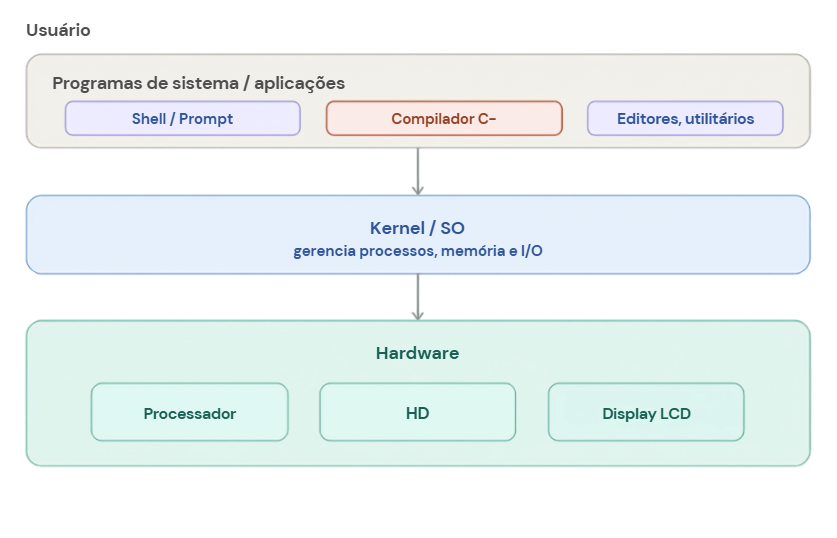
\includegraphics[width=0.8\textwidth]{Figuras/camadas.png}
  \fonte{Adaptado de \citeonline{tanenbaum2016}.}
\end{figure}
 
Esta disciplina propõe a construção de um sistema computacional completo em etapas
encadeadas. Nas fases anteriores foram desenvolvidos um processador RISC-V RV32IM
monociclo e um compilador para a linguagem C-. Sobre essa base, o presente trabalho
trata da etapa seguinte: o projeto do sistema operacional que executará sobre esse
processador e cujos programas serão escritos e compilados na linguagem de alto nível
já disponível. Trata-se, portanto, de integrar hardware e software em torno de um
mesmo objetivo.
 
O estudo de sistemas operacionais é motivado justamente por essa posição central:
compreender como um SO gerencia processos, memória, arquivos e dispositivos é o que
permite transformar um processador funcional em uma máquina de uso geral, capaz de
executar múltiplos programas de forma coordenada. Este relatório concentra-se na
\emph{especificação} desse projeto, isto é, na definição fundamentada das técnicas e
dos algoritmos que guiarão a implementação nas etapas posteriores.


% ==========================================================
\chapter{Objetivos}
% ==========================================================
\section{Geral}
Projetar um sistema operacional completo, com gerenciamento de processos, de memória,
de sistema de arquivos e de dispositivos de entrada e saída, capaz de executar sobre o
processador RISC-V RV32IM e o compilador da linguagem C- desenvolvidos nos laboratórios
anteriores, tendo como alvo o kit FPGA DE2-115.
 
\section{Específico}
Para alcançar o objetivo geral, esta etapa tem como metas específicas:
\begin{itemize}
  \item Realizar o levantamento teórico das quatro áreas de gerenciamento de um SO:
        processos, memória, sistema de arquivos e dispositivos de E/S.
  \item Especificar o gerenciamento de processos por meio de escalonamento circular
        (\emph{round-robin}) com preempção por temporizador, apoiado em um mecanismo
        de interrupção adaptado à arquitetura RV32IM, sem seguir a especificação
        privilegiada do RISC-V, devido à sua complexidade.
  \item Especificar o gerenciamento de memória por particionamento fixo, com
        partições de tamanho igual para o SO e para até dez processos de usuário.
  \item Especificar o sistema de arquivos, provendo ao menos a criação, a renomeação
        e a eliminação de programas armazenados no HD.
  \item Especificar o gerenciamento de dispositivos de E/S de forma modularizada,
        abrangendo as chaves, o display de sete segmentos e o HD simulado.
  \item Especificar a BIOS, responsável pela inicialização do sistema e pelo
        carregamento do SO a partir do HD.
  \item Especificar um \emph{shell} que permita executar um programa isoladamente,
        executar até dez programas com preempção, e criar, renomear e eliminar
        programas.
  \item Descrever, de forma integrada, o funcionamento do SO como uma unidade,
        modelando a interligação entre os quatro gerenciamentos.
  \item Especificar as alterações e inclusões de hardware e de software, herdadas dos
        laboratórios anteriores, necessárias à execução do SO.
\end{itemize}
 
% ==========================================================
\chapter{Fundamentação Teórica}
% ==========================================================
\section{Gerenciamento de Processos}
Um processo é a abstração de um programa em execução, incluindo seu contador de
programa, seus registradores e as variáveis que manipula \cite{tanenbaum2016}. Como um
único processador executa uma instrução por vez, a sensação de que vários programas
avançam simultaneamente é uma ilusão sustentada pelo sistema operacional, que alterna a
CPU entre os processos com rapidez. Cada processo pode encontrar-se em três estados
básicos: em execução, quando ocupa a CPU; pronto, quando poderia executar mas aguarda
sua vez; e bloqueado, quando não pode prosseguir até que algum evento externo ocorra,
como a conclusão de uma operação de entrada e saída.

A escolha de qual processo pronto recebe a CPU cabe ao escalonador, e a política que
ele segue depende do tipo de ambiente. Em sistemas em lote costuma-se usar algoritmos
não preemptivos, como o primeiro a chegar é o primeiro a ser servido, ou a tarefa mais
curta primeiro. Em sistemas interativos, ao contrário, é desejável que nenhum processo
monopolize o processador, o que torna a preempção necessária \cite{silberschatz2015}.
Entre as políticas interativas estão o escalonamento por prioridades, o escalonamento
por loteria e o chaveamento circular.

No chaveamento circular, ou \emph{round-robin}, atribui-se a cada processo uma fatia de
tempo chamada \emph{quantum}. Enquanto executa, o processo consome seu quantum; se ele
se esgota antes de o processo terminar, o escalonador realiza a preempção e transfere a
CPU ao próximo da fila, colocando o processo interrompido no final dela. Caso o processo
seja bloqueado ou termine antes do fim do quantum, a troca ocorre de imediato. A grande
vantagem do método é a simplicidade: basta manter uma única fila de processos prontos.
A troca de um processo por outro, chamada troca de contexto, consiste em salvar os
registradores e o contador de programa do processo que deixa a CPU e restaurar os do
processo que assume, de modo que cada um retome a execução exatamente de onde parou.
A escolha do quantum envolve um compromisso: valores muito pequenos aumentam a
frequência de trocas e, com ela, o custo de processamento desperdiçado; valores muito
grandes prejudicam o tempo de resposta \cite{tanenbaum2016}.

A troca de contexto depende de uma estrutura que o SO mantém para cada processo:
o bloco de controle de processo (PCB). Nele ficam registradas as informações
necessárias para retomar a execução mais tarde: o estado do processo, o contador
de programa, o conteúdo dos registradores e os dados sobre a memória ocupada. O
conjunto de todos os PCBs compõe a tabela de processos do sistema
\cite{silberschatz2015}.

\section{Gerenciamento de Memória}
Cabe ao gerenciador de memória controlar quais partes da memória estão ocupadas e
quais estão livres, alocando espaço aos processos que o requisitam e liberando-o quando
esses processos terminam \cite{tanenbaum2016}. Em um ambiente com multiprogramação, mais
de um processo ocupa a memória ao mesmo tempo, o que levanta dois problemas: a
realocação, já que um processo não sabe de antemão em que endereço será carregado, e a
proteção, para que um processo não acesse a área de outro. Ambos costumam ser resolvidos
com o uso de um registrador base, que desloca todos os endereços do processo, e de um
registrador limite, que delimita sua fronteira.

A forma mais simples de organizar a memória com multiprogramação é o particionamento
fixo, em que a memória é dividida previamente em partições, e cada partição recebe
exatamente um processo. O grau de multiprogramação fica limitado ao número de
partições. Quando as partições têm tamanho igual, o processo que não ocupa toda a
sua partição deixa espaço sem uso dentro dela, fenômeno chamado fragmentação interna.
Já no particionamento variável, cada processo recebe apenas o espaço de que precisa,
o que elimina a fragmentação interna, mas gera fragmentação externa: com o tempo,
a memória livre fica dividida em buracos pequenos demais para novos processos
\cite{silberschatz2015}.

Para acompanhar a ocupação da memória, duas estruturas são comuns: o mapa de bits,
em que cada unidade de alocação corresponde a um bit que indica se ela está livre ou
ocupada, e a lista encadeada de segmentos livres e ocupados. Sobre essas estruturas
operam algoritmos de alocação como o \emph{first-fit}, que escolhe o primeiro espaço livre
grande o bastante, além de variações como o \emph{best-fit} e o \emph{worst-fit}
\cite{silberschatz2015}. Quando a memória disponível não é suficiente para todos os
processos ativos, pode-se recorrer ao \emph{swapping}, que transfere um processo inteiro
para o disco e o traz de volta mais tarde.

Uma solução mais sofisticada é a memória virtual, geralmente implementada por paginação.
Nela, o espaço de endereçamento de cada processo é dividido em páginas de tamanho fixo,
mapeadas para molduras na memória física por uma unidade de gerenciamento de memória,
que traduz endereços virtuais em endereços reais. Quando uma página referenciada não
está presente na memória, ocorre uma falta de página, e o sistema a busca no disco. Isso
permite executar programas maiores que a memória principal, ao custo de decidir qual
página remover quando não há molduras livres, tarefa dos algoritmos de substituição, como
o FIFO, a segunda chance, o relógio e o LRU \cite{tanenbaum2016}.

\section{Gerenciamento de Sistema de Arquivos}
Arquivos são a forma como o sistema operacional armazena informação de maneira
persistente, isto é, de modo que ela sobreviva ao término dos processos e ao desligamento
da máquina \cite{tanenbaum2016}. O sistema de arquivos define como os arquivos são
nomeados, estruturados, acessados, protegidos e implementados sobre o dispositivo de
armazenamento, escondendo do usuário os detalhes físicos do disco. Quanto à estrutura
interna, um arquivo pode ser visto como uma sequência de bytes, abordagem mais comum
por sua flexibilidade, como uma sequência de registros de tamanho fixo, ou como uma
árvore de registros indexados por uma chave.

Sobre os arquivos, o SO oferece um conjunto de operações, entre elas a criação, a
eliminação, a leitura, a escrita e a renomeação \cite{tanenbaum2016}.

Além dos arquivos regulares, o sistema mantém diretórios, que organizam os arquivos e
associam cada nome à informação necessária para localizá-lo no disco. A maneira como os
blocos de um arquivo são dispostos no dispositivo caracteriza o método de alocação. Na
alocação contígua, os blocos ficam em sequência, o que favorece a leitura mas gera
fragmentação. Na alocação por lista encadeada, cada bloco aponta para o próximo,
eliminando a fragmentação externa ao preço de tornar lento o acesso aleatório. Uma
variação mantém esses ponteiros em uma tabela na memória, a exemplo da tabela de
alocação de arquivos (FAT), enquanto a abordagem por i-node associa a cada arquivo uma
estrutura que lista seus blocos e só precisa estar carregada quando o arquivo está em uso
\cite{silberschatz2015}.

\section{Gerenciamento de Dispositivos de E/S}
O gerenciamento de entrada e saída tem por objetivo controlar os dispositivos e oferecer
aos programas uma interface uniforme, independente das particularidades de cada
\emph{hardware} \cite{tanenbaum2016}. Fisicamente, cada dispositivo é operado por um
controlador, que expõe um conjunto de registradores por meio dos quais a CPU envia
comandos e lê o estado do dispositivo. Quando esses registradores são acessados como se
fossem posições de memória, fala-se em entrada e saída mapeada em memória, esquema que dispensa instruções
especiais de E/S.

Há três formas principais de conduzir uma operação de E/S. Na E/S programada, a CPU fica em espera ocupada, consultando repetidamente o
estado do dispositivo até que ele esteja pronto, o que é simples, mas desperdiça
ciclos de processamento. Na E/S orientada a interrupções, a CPU inicia a operação
e passa a executar outra tarefa, e o dispositivo sinaliza a conclusão por meio de
uma interrupção. Por fim, no acesso direto à memória (DMA), um controlador
dedicado transfere os dados entre o dispositivo e a memória sem intervenção da
CPU, que só é notificada ao fim da transferência \cite{tanenbaum2016}.

Para lidar com a diversidade de dispositivos, o software de E/S é organizado em
camadas: na base estão os tratadores de interrupção; acima deles, os \emph{drivers},
que concentram o código específico de cada dispositivo; em seguida, o software de
E/S independente de dispositivo, que oferece aos programas uma interface uniforme;
e, no topo, as bibliotecas e programas de usuário. Essa modularização permite
acrescentar ou alterar um dispositivo modificando apenas o seu \emph{driver}, sem
impacto sobre o restante do sistema \cite{tanenbaum2016}.

A inicialização do sistema é conduzida pela BIOS, programa armazenado em memória
não volátil na placa-mãe. Ao ligar o computador, a BIOS verifica os componentes do
sistema, identifica o dispositivo de inicialização e lê dele um setor fixo que
contém o programa responsável por carregar o SO na memória principal, transferindo
em seguida a execução para ele \cite{tanenbaum2016}.
 
% ==========================================================
\chapter{Desenvolvimento}
\label{cap:desenvolvimento}
% ==========================================================
 
\section{Alterações nas Plataformas de Hardware e Software}
A Figura~\ref{fig:datapath} apresenta o \emph{datapath} do processador RV32IM
\cite{patterson2014} desenvolvido no laboratório de Arquitetura, ponto de partida
para as alterações descritas nesta seção.

\begin{figure}[H]
  \centering
  \caption{\emph{Datapath} atual do processador RV32IM}
  \label{fig:datapath}
  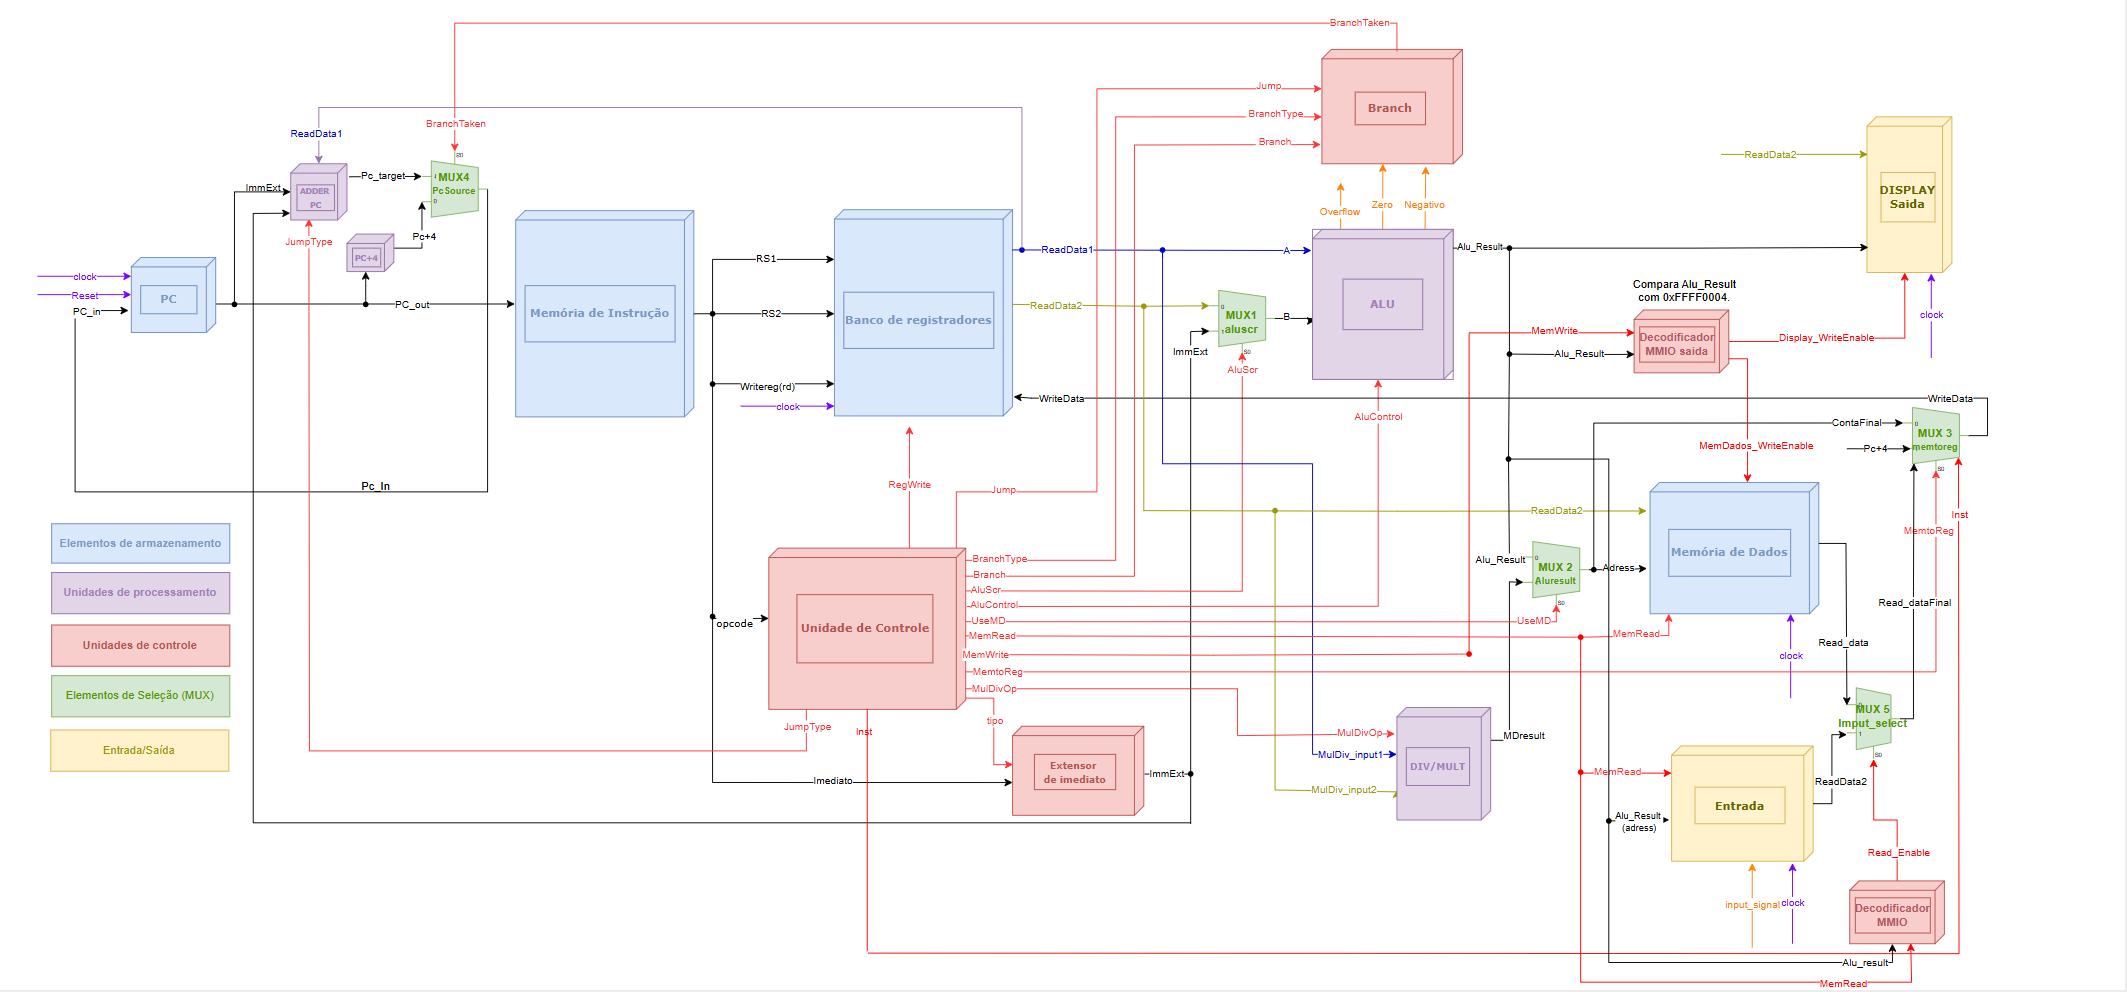
\includegraphics[width=\textwidth]{Figuras/datapath.png}
  \fonte{Autoria própria.}
\end{figure}

As decisões de projeto implicam um conjunto de alterações na plataforma de hardware
herdada do laboratório de Arquitetura. A memória de instruções, hoje implementada como
ROM de 512 posições, precisará tornar-se gravável e ser ampliada para 7168 palavras,
divididas em 11 partições: 2048 palavras reservadas ao SO e dez partições de 512
palavras, uma para cada processo de usuário, de modo que o código de cada processo
seja carregado do HD uma única vez, na sua criação. A memória de dados será expandida
de 2048 para 2816 palavras. Além disso, será incluído
um temporizador, responsável por gerar as interrupções de \emph{quantum}, e a lógica
de tratamento de interrupção no \emph{datapath}, responsável por salvar o contador de
programa e desviar a execução para uma rotina de tratamento fixa. Os endereços de E/S
mapeados em memória serão realocados para fora da faixa da memória de dados, o que
exige apenas a atualização das constantes comparadas pelos decodificadores. Completam
esse conjunto o disco rígido emulado, a BIOS, um \emph{display} de cristal
líquido (LCD) alfanumérico dedicado a mensagens de texto sobre o estado do SO
(cuja implementação seguirá o protocolo padrão do controlador HD44780, consultando-se
como referência um projeto de controle de LCD já disponível para o kit DE2-115
\cite{lcdde2115}), e as instruções dedicadas de transferência entre o HD e as
memórias, detalhados na Seção~\ref{sec:es}. O
gerenciamento de sistema de arquivos acrescenta a essa lista apenas uma
estrutura de \emph{software}: a tabela de diretório de tamanho fixo (48
palavras, para até 16 programas), gravada em uma região reservada do próprio HD
emulado e manipulada pelas rotinas de criação, renomeação e eliminação de
programas do SO, sem exigir nenhum módulo de \emph{hardware} adicional além do
já previsto para o HD (Seção~\ref{sec:arquivos}).

 
\section{Gerenciamento de Processos}
O gerenciamento de processos adotará escalonamento circular (\emph{round-robin}) com
preempção por temporizador. Cada processo recebe uma fatia de tempo (\emph{quantum})
fixa; ao esgotá-la, o temporizador dispara uma interrupção que devolve o controle ao
SO, o qual salva o contexto do processo interrompido e escala o próximo processo da
fila de prontos. Um processo também pode ceder a CPU voluntariamente antes do fim do
seu \emph{quantum}, ao sinalizar seu término.
 
O mecanismo de interrupção será \emph{adaptado} à arquitetura RV32IM, sem seguir a
especificação privilegiada do RISC-V (CSRs, \texttt{mtvec}, \texttt{mepc},
\texttt{mret}) \cite{riscvpriv2021}. Em vez disso, empregar-se-á um esquema simplificado: um registrador
dedicado guarda o contador de programa no instante da interrupção, um endereço fixo
identifica a rotina de tratamento e instruções próprias controlam a habilitação da
preempção e o retorno da interrupção. Essa escolha reduz substancialmente a
complexidade de hardware sem prejuízo para os objetivos do projeto.

A garantia de que o próprio SO nunca é interrompido depende de uma flag de um bit,
mantida no \emph{datapath}, que habilita ou desabilita a contagem do temporizador.
Uma instrução dedicada (\texttt{set\_multiprog}) liga essa flag, e o SO a executa
apenas imediatamente antes de saltar para a partição de um processo de usuário.
Enquanto a flag permanece em zero, o contador do temporizador fica parado, de modo
que a interrupção de \emph{quantum} é fisicamente impossível durante a execução do
SO. Ao atingir o valor do \emph{quantum}, o próprio \emph{hardware} desliga a flag,
salva o contador de programa e desvia a execução para o SO. O SO só a religa ao
despachar o próximo processo, fechando um ciclo em que a preempção nunca alcança o
código do SO. A Figura~\ref{fig:flagpreempcao} ilustra essas duas fases. O mesmo
mecanismo cobre a execução sem preempção prevista para o \emph{shell}: basta não
ligar a flag antes de saltar para o processo, que então roda até o fim sem risco de
interrupção.

\begin{figure}[H]
  \centering
  \caption{Habilitação e desabilitação da preempção}
  \label{fig:flagpreempcao}
  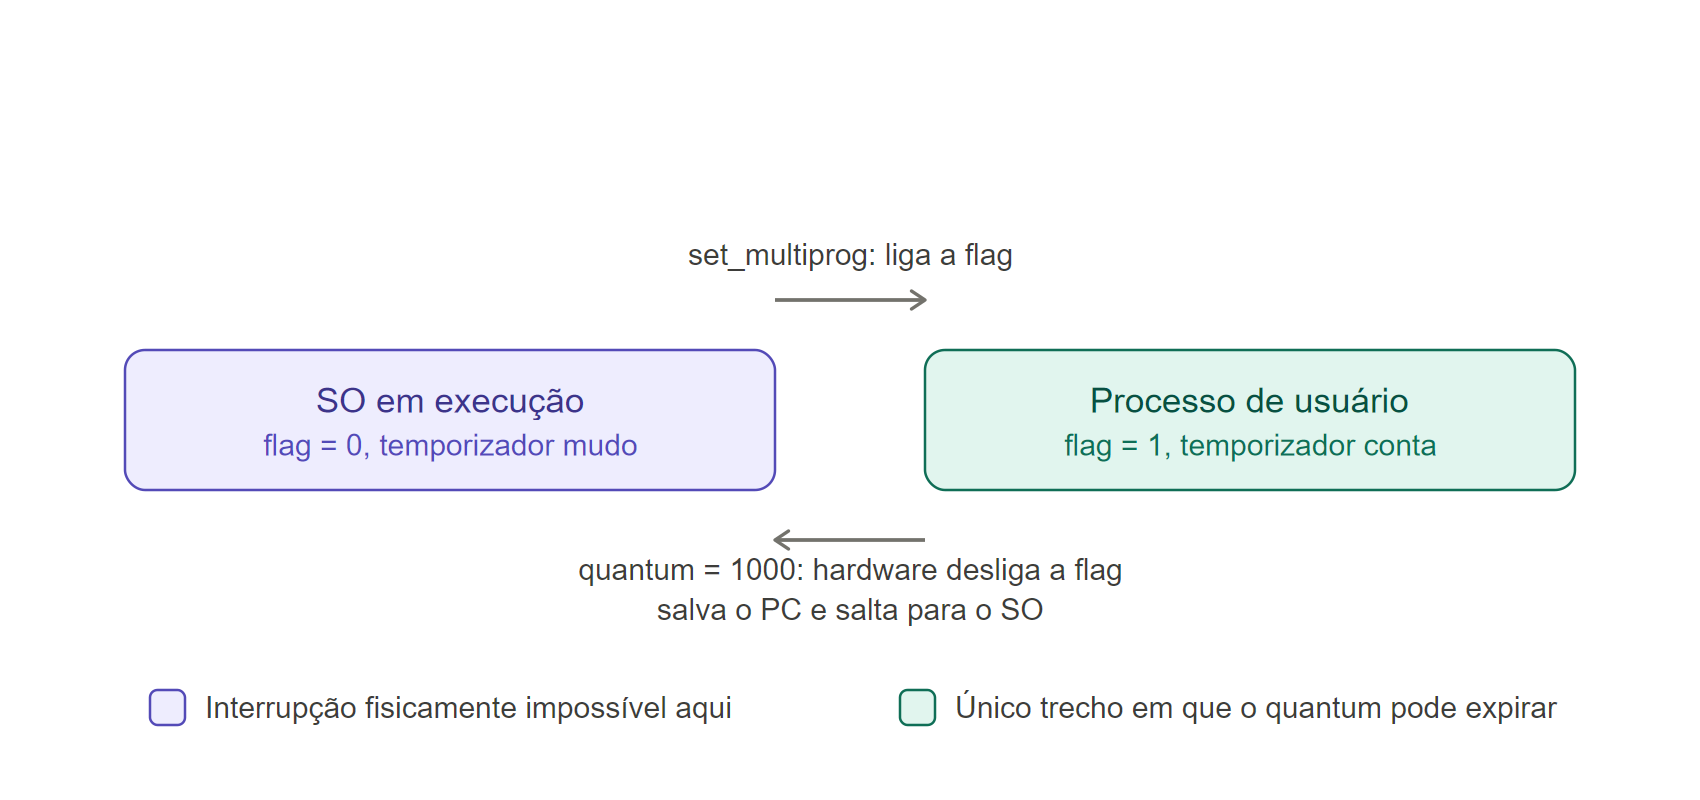
\includegraphics[width=0.85\textwidth]{Figuras/flagpreempcao.png}
  \fonte{Autoria própria.}
\end{figure}

A fila de prontos é representada por um vetor de dez posições, uma para cada
partição de usuário, cada uma marcada como livre ou ocupada. Um ponteiro indica a
partição em execução e avança de forma circular entre as posições ocupadas a cada
troca de contexto, sem exigir lista encadeada ou outra estrutura dinâmica, já que
cada processo já ocupa uma partição de índice fixo.

A troca de contexto consiste em salvar o conjunto de registradores do processo
interrompido na \emph{zona de troca}, uma área reservada dentro da própria
partição de dados do processo, e
restaurar os registradores do processo a ser escalonado, retomando sua execução a
partir do contador de programa previamente salvo.

O valor do \emph{quantum} foi fixado em \textbf{1000 ciclos de clock}. A troca de
contexto salva e restaura os 31 registradores de uso geral (\texttt{x1}--\texttt{x31})
com uma instrução \texttt{sw}/\texttt{lw} por registrador: 31 armazenamentos mais 31
carregamentos totalizam 62 ciclos no processador monociclo, aos quais se somam as
demais instruções de controle da rotina de troca, resultando em um custo aproximado
de 70 ciclos. Esse custo não inclui
recarregar o código do processo a partir do HD, pois cada processo mantém residente
sua própria partição de memória de instrução após a primeira carga (Seção~\ref{sec:es}). Assim, um \emph{quantum} de 1000 ciclos mantém o custo da troca em torno de
7\% do tempo total ($70/1000$), abaixo dos 10\% considerados aceitáveis, em linha
com a recomendação de que o \emph{quantum} seja grande em relação ao tempo de troca
de contexto \cite{silberschatz2015}.

O processador opera a 500\,Hz, resultado de dividir o \emph{clock} de 50\,MHz da
placa por 100.000. Nessa frequência, um \emph{quantum} de 1000 ciclos equivale a 2
segundos por fatia de tempo, o suficiente para observar várias trocas de contexto
ao longo da demonstração do sistema.

A Figura~\ref{fig:filaprontos} ilustra a fila circular de processos prontos e a
sequência de passos executada quando o \emph{quantum} do processo em execução se
esgota.

\begin{figure}[H]
  \centering
  \caption{Fila de prontos e fluxo de troca de contexto}
  \label{fig:filaprontos}
  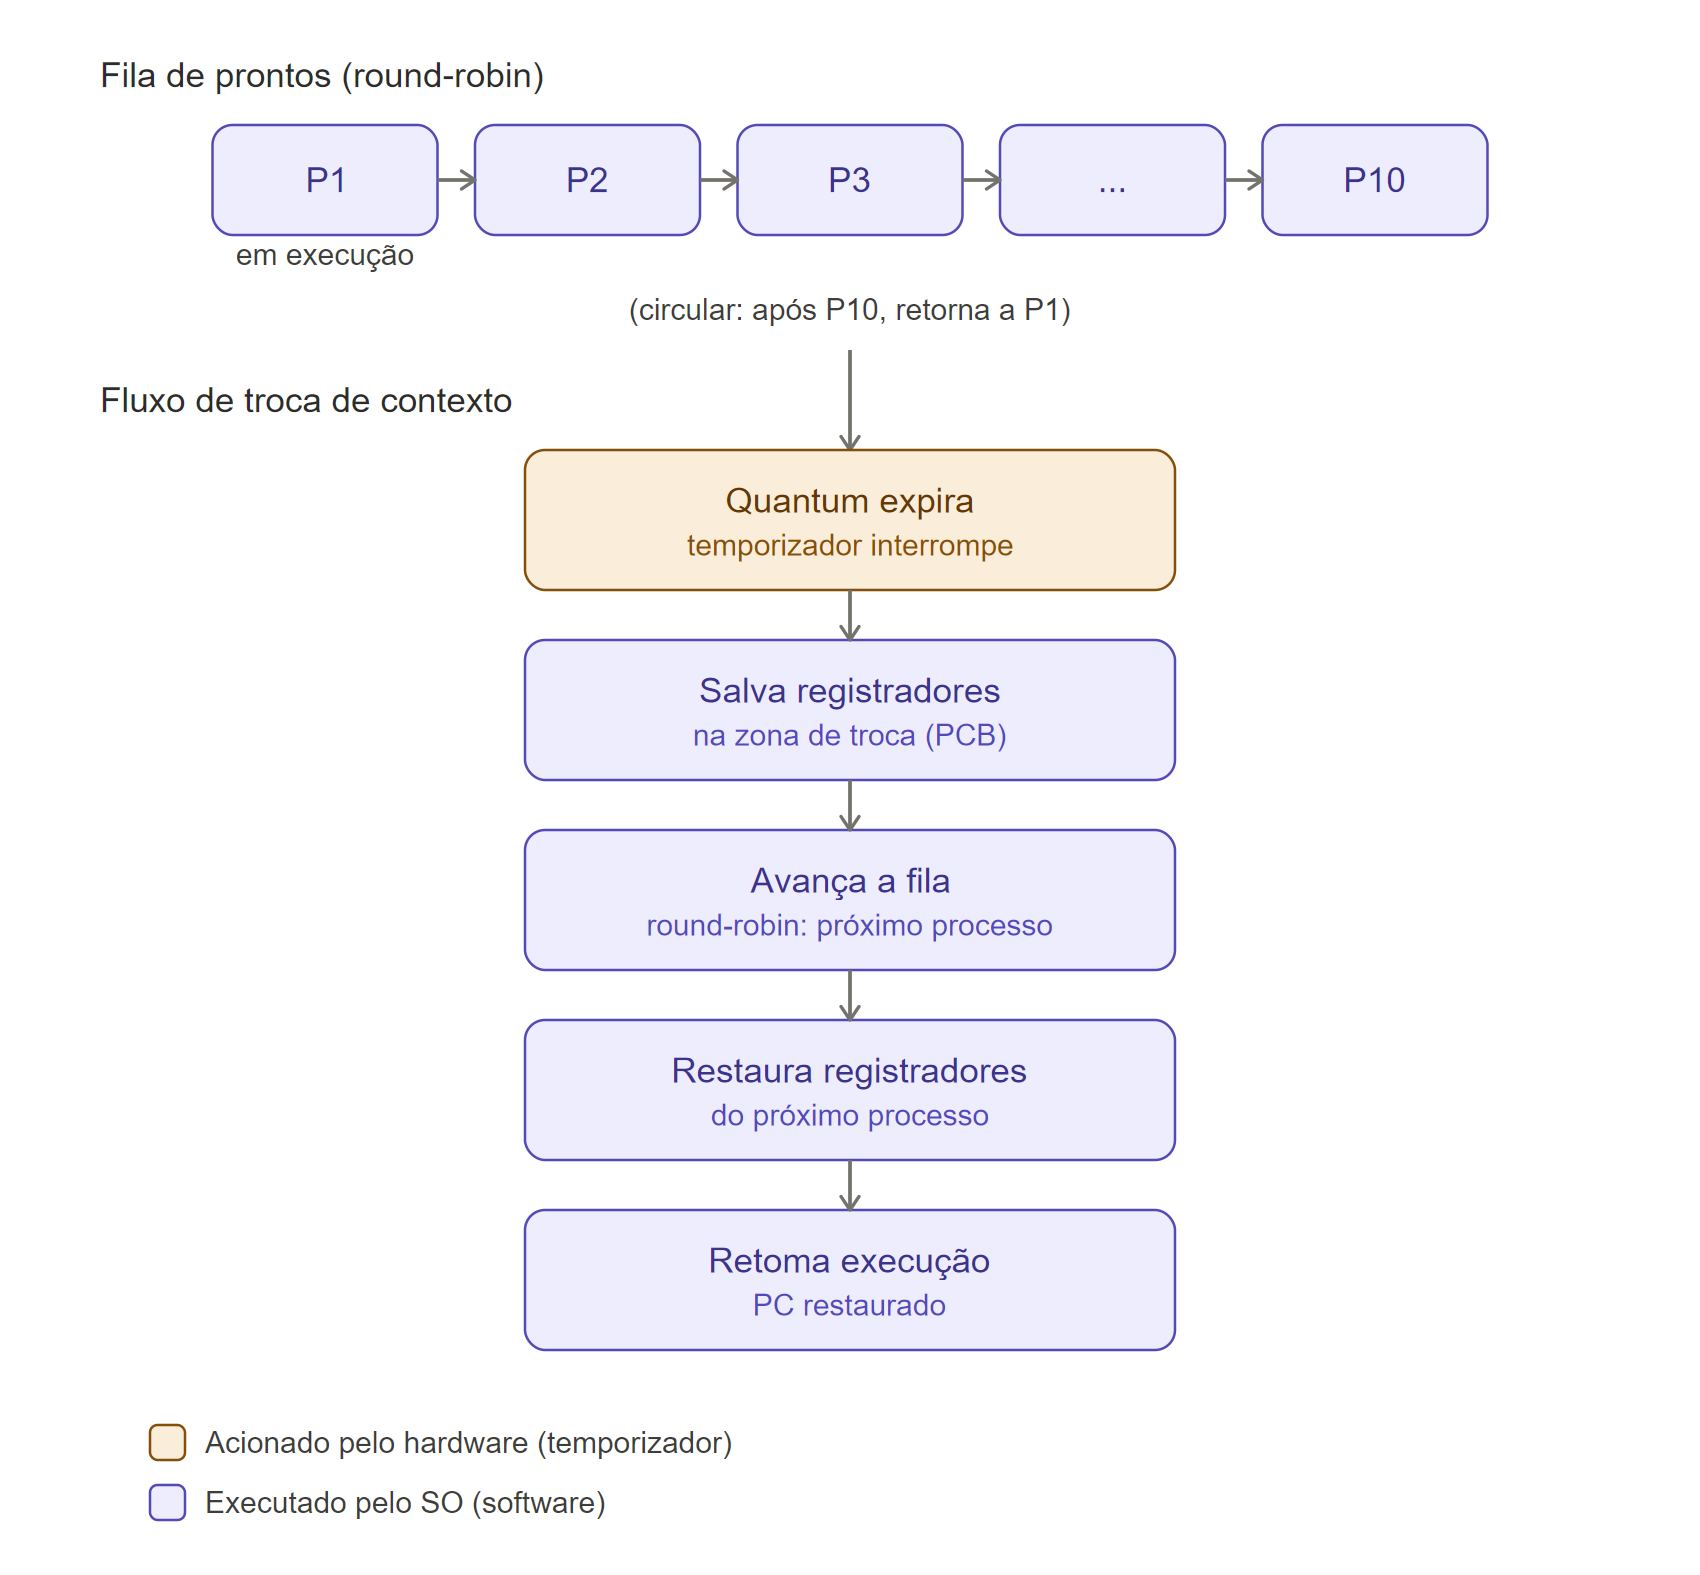
\includegraphics[width=0.85\textwidth]{Figuras/filaprontos.png}
  \fonte{Autoria própria.}
\end{figure}
 
\section{Gerenciamento de Memória}
Adota-se o particionamento fixo com partições de tamanho igual. A memória de dados,
originalmente com 2048 palavras, será expandida para 2816 palavras e dividida em 11
partições de 256 palavras: a partição 0 é reservada ao SO e as partições 1 a 10 aos
processos de usuário, respeitando o limite de dez processos simultâneos do projeto.

O tamanho das partições foi definido a partir do uso de pilha medido por simulação
nos dez programas de teste da etapa anterior. O pior caso, o cálculo recursivo de
\texttt{fib(9)}, ocupou 148 palavras. Adotou-se a potência de 2 imediatamente
superior, o que preserva margem para programas futuros e permite obter o endereço
físico por deslocamento de bits, sem uso de multiplicador:
\begin{equation}
  \text{endereço} = (\text{índice} \ll 8) \mid \text{deslocamento}
\end{equation}

Como cada partição tem posição e tamanho fixos, não é necessário manter mapa de bits
nem lista de espaços livres: basta ao SO registrar quais índices estão ocupados. O
custo é a fragmentação interna, já que um processo pequeno ocupa a partição inteira.
Técnicas como paginação e \emph{swapping} foram descartadas por exigirem uma unidade
de gerenciamento de memória e acessos frequentes ao disco, o que aumentaria a
complexidade do hardware sem ganho para o conjunto de programas previsto.

A memória de instruções segue o mesmo particionamento fixo, mas com uma diferença
importante: a partição do SO não tem o mesmo tamanho das partições de usuário. O
próprio SO reúne escalonador, rotina de troca de contexto, tabela de diretório e
\emph{shell}, um volume de código que tende a superar facilmente uma partição de 512
palavras. Por isso, a partição do SO recebe 2048 palavras, o mesmo teto já reservado
para o SO no HD emulado (Seção~\ref{sec:arquivos}), enquanto as dez partições de
usuário mantêm 512 palavras cada, preservando o cálculo de endereço por deslocamento
de bits nessas partições. A memória de instruções passa, assim, de 512 para 7168
palavras (2048 do SO mais dez partições de 512).

Somadas, as memórias de dados (2816 $\times$ 32 bits = 90.112 bits) e de instruções
(7168 $\times$ 32 bits = 229.376 bits) totalizam 319.488 bits, ou 312 Kbits. O
processador RV32IM é sintetizado no chip Cyclone IV E EP4CE115 do kit DE2-115, que
dispõe de 3.888 Kbits de memória embarcada \cite{intelep4ce115}. As duas memórias
juntas ocupam, portanto, cerca de 8,0\% dessa capacidade ($312/3888$).
\section{Gerenciamento de Sistema de Arquivos}
\label{sec:arquivos}

Adota-se a alocação contígua como método de organização dos programas de usuário
no HD emulado, com uma tabela de diretório em posição fixa, situada logo após a
região reservada ao SO (Seção~\ref{sec:es}). Essa escolha decorre diretamente da
decisão de tamanho fixo por \emph{slot} já adotada para o carregamento de
programas: como cada entrada de diretório corresponde a um bloco de tamanho
conhecido, dispensam-se as estruturas usuais de alocação com tamanho variável,
como a lista encadeada ou a tabela de alocação de arquivos (FAT). A principal
vantagem dessas estruturas sobre a alocação contígua, evitar a fragmentação
externa entre arquivos de tamanhos distintos, perde relevância quando todos os
arquivos possuem exatamente o mesmo tamanho \cite{silberschatz2015}.

O HD emulado organiza-se em três regiões consecutivas: o SO, do endereço 0 até a
constante de tamanho fixo conhecida pela BIOS (Seção~\ref{sec:es}); a tabela de
diretório, logo em seguida; e a área de programas, com 16 posições de 400
palavras cada. O limite de 16 programas armazenáveis foi fixado acima do número máximo de
processos executáveis simultaneamente (dez), de modo a permitir
a criação e a remoção de programas sem esgotar rapidamente o espaço de
armazenamento.

Como a posição de cada \emph{slot} é determinada unicamente pelo seu índice na
tabela,
\begin{equation}
  \text{endereço do \emph{slot}} = \text{TAMANHO\_SO} + \text{índice} \times 400,
\end{equation}
cada entrada de diretório dispensa os campos de início e tamanho normalmente
exigidos pela alocação contígua, reduzindo-se a um nome de até oito caracteres e
um sinalizador de ocupação: três palavras ao todo. A tabela completa ocupa,
portanto, 48 palavras (16 $\times$ 3), quantidade desprezível frente às regiões
de memória de dados e de instrução.

As operações mínimas exigidas do sistema de arquivos (criar, renomear e
eliminar um programa) resumem-se, nessa organização, a operações sobre a
tabela de diretório. Para renomear, atualiza-se apenas o campo de nome da
entrada; para eliminar, zera-se o sinalizador de ocupação, sem necessidade de
apagar fisicamente o conteúdo do \emph{slot}, que será sobrescrito na próxima
criação.

A criação de um programa depende de como seu código chega ao sistema, e aqui
pesa uma limitação já discutida: o único mecanismo de entrada disponível é o
\texttt{input()} via chaves e botão de confirmação (Seção~\ref{sec:es}), sem
teclado para digitar código-fonte. Adota-se, por isso, a entrada manual do
código já compilado: o usuário informa o nome do novo programa e, em seguida,
cada palavra de seu código, uma de cada vez, pelas chaves. O SO grava o par
nome/ocupado na primeira entrada livre da tabela de diretório e escreve as
palavras recebidas no \emph{slot} correspondente. Essa forma de criação
restringe-se, na prática, a programas curtos, de poucas instruções, dado o
custo de inserir cada palavra manualmente pelas chaves.

\section{Gerenciamento de Dispositivos de E/S}
\label{sec:es}

\subsection{Acesso ao HD e inicialização do sistema}

O processador desenvolvido segue uma arquitetura Harvard, com memória de instrução e
memória de dados separadas. Na configuração atual, a memória de instrução é somente de
leitura (ROM), acessada exclusivamente pelo contador de programa durante a busca. Para
que o SO possa carregar programas em tempo de execução, é necessário que essa memória
passe a aceitar escrita e que exista um dispositivo de armazenamento persistente, o HD,
de onde os programas serão trazidos.

Duas abordagens foram consideradas. Na primeira, o HD e a memória de instrução seriam
mapeados no mesmo espaço de endereços da memória de dados, permitindo reutilizar as
instruções \texttt{lw} e \texttt{sw} nas transferências. Na segunda, o HD e a memória de
instrução seriam mantidos como módulos independentes, fora do espaço de endereçamento
comum, com instruções dedicadas para as transferências entre eles.

Optou-se pela segunda abordagem. Primeiro, pelo isolamento: como o HD e a memória de
instrução não pertencem ao espaço acessível por \texttt{sw}, um \emph{store} emitido por
um processo, ainda que com endereço incorreto, não alcança essas regiões, e a proteção
do SO e do código carregado passa a ser garantida pela própria arquitetura. Segundo, por
preservar a organização Harvard já implementada, enquanto a abordagem mapeada exigiria
unificar as memórias ou criar uma ponte entre elas, além de lógica de proteção por faixa
de endereço. Terceiro, por se tratar de um caminho já validado em projetos anteriores da
disciplina. O custo é a inclusão de novas instruções no processador, com os respectivos
casos na unidade de controle: transferência do HD para a memória de instrução,
transferência entre o HD e a memória de dados, e troca da fonte de busca de instruções.

A inicialização fica a cargo de uma BIOS implementada como memória ROM independente,
pré-carregada com o código de partida e utilizada como fonte de busca no instante
inicial. Cabem a ela o teste de partida, a identificação do HD, a cópia do SO para a
memória de instrução e a transferência da execução para o SO. O SO ocupa as primeiras
posições do HD, do endereço 0 até uma constante fixa de tamanho conhecida pela BIOS,
de forma análoga ao setor de inicialização dos computadores convencionais. Concluída a
cópia, uma instrução dedicada alterna a fonte de busca da BIOS para a memória de
instrução, dando início à execução do SO. Esse fluxo é ilustrado na
Figura~\ref{fig:boot}.

\begin{figure}[H]
  \centering
  \caption{Fluxo de inicialização do sistema}
  \label{fig:boot}
  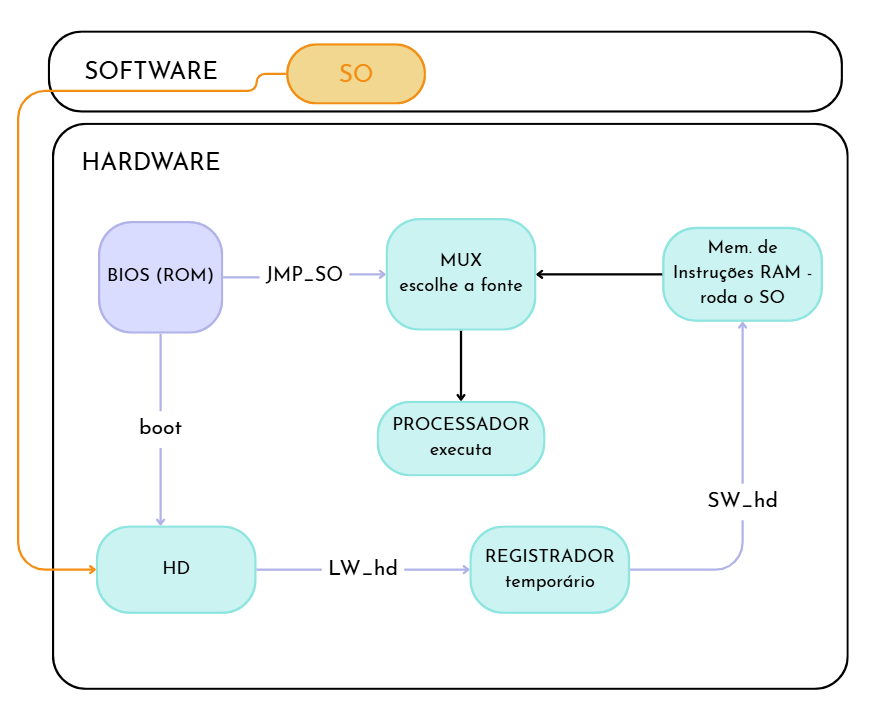
\includegraphics[width=0.85\textwidth]{Figuras/boot.png}
  \fonte{Autoria própria.}
\end{figure}

\subsection{Entrada e saída de dados}

As chaves e o display são acessados por E/S mapeada em memória, por meio das funções
\texttt{input()} e \texttt{output()} da linguagem C-. Originalmente, esses dispositivos
ocupavam os endereços 2044 e 2040, que, com a expansão da memória de dados para 2816
palavras, passariam a coincidir com a partição 7. Como o processador não dispõe da
instrução \texttt{lui}, necessária para montar constantes de 32 bits
\cite{riscvunpriv2019}, os dispositivos
foram realocados para os deslocamentos $-4$ e $-8$ relativos ao registrador
\texttt{x0}. A extensão de sinal do imediato, já existente no \emph{datapath}, converte
esses valores nos endereços \texttt{0xFFFFFFFC} (entrada) e \texttt{0xFFFFFFF8} (saída),
fora de qualquer faixa de memória do sistema, sem necessidade de \emph{hardware}
adicional além da atualização dos decodificadores.

Na entrada, o usuário ajusta o valor nas chaves e pressiona o botão de confirmação.
Um circuito de \emph{debounce} filtra o ruído mecânico do botão, e a detecção da borda
de subida captura o valor das chaves e sinaliza que há um dado disponível. Enquanto
esse sinal não é ativado, uma leitura no endereço de entrada mantém o contador de
programa travado, de modo que o processador aguarda o dado em \emph{hardware}, sem
laço de consulta em \emph{software}. Na saída, uma escrita no endereço do display
habilita o registro do valor a ser exibido.

Adota-se, portanto, a E/S programada para todos os dispositivos, sem controlador de
DMA e sem interrupções de dispositivo. Vale notar que essa classificação não implica
espera ocupada em \emph{software}: o próprio \emph{hardware} mantém o contador de
programa bloqueado até que o dado esteja disponível, dispensando qualquer laço de
consulta explícito no código do SO. Essa escolha mantém o \emph{hardware} simples,
mas impõe uma limitação: como o travamento do contador de programa não é interrompido
pelo temporizador, um processo que aguarda entrada impede a preempção e bloqueia a
execução de todos os demais até que o dado seja confirmado. O tratamento da entrada
por interrupção, que eliminaria essa limitação, ficou fora do escopo deste projeto.

Além do \emph{display} de sete segmentos, já herdado dos laboratórios anteriores e
limitado a valores numéricos, inclui-se um \emph{display} de cristal líquido (LCD)
alfanumérico, mapeado em memória em um terceiro endereço dedicado ($-12$, estendido
para \texttt{0xFFFFFFF4} pelo mesmo mecanismo de sinal descrito acima). Cada escrita
nesse endereço envia um caractere, cujo código ASCII é convertido para exibição pelo
próprio \emph{hardware} do LCD; um contador de posição, mantido no \emph{datapath},
avança automaticamente a cada caractere escrito e retorna ao início da tela ao
alcançar seu limite, de modo que o SO escreve uma mensagem completa com uma
sequência de chamadas a \texttt{output()}, sem precisar calcular posições.

O LCD permite ao SO comunicar seu estado ao usuário sem depender da interpretação
de códigos em LEDs ou de valores numéricos no \emph{display} de sete segmentos:
a etapa da BIOS em andamento durante o \emph{boot}, o nome do programa em execução
a cada troca de contexto e o tipo de dado esperado quando o sistema aguarda uma
entrada são exibidos como texto, atualizados pela mesma rotina de escrita que
concentra o acesso ao dispositivo (Seção~\ref{sec:integracao}).

Em conformidade com a organização em camadas do software de E/S, o acesso a cada
dispositivo é concentrado em rotinas próprias do SO: leitura das chaves, escrita no
\emph{display} de sete segmentos, escrita de mensagens no LCD e transferência de
blocos entre o HD e as memórias. O \emph{shell} e as
demais partes do SO acessam os dispositivos apenas por meio dessas rotinas, de modo
que a alteração de um dispositivo exige modificar somente a rotina correspondente.


\section{Integração dos Gerenciamentos}
\label{sec:integracao}

Os quatro gerenciamentos especificados nas seções anteriores não operam de forma
isolada: cada evento relevante do sistema aciona, em sequência, mecanismos de mais
de uma área. A Figura~\ref{fig:integracao} ilustra essa interligação a partir do
ciclo de vida de um processo, do momento em que seu programa é criado no HD até sua
eventual conclusão.

A criação de um programa é uma operação exclusiva do gerenciamento de sistema de
arquivos: o shell grava um novo par nome/ocupado na tabela de diretório e reserva o
\emph{slot} de 400 palavras correspondente na área de programas do HD. A execução,
por sua vez, aciona o gerenciamento de processos, que insere o programa na fila de
prontos do escalonador circular. Ao ser escalado pela primeira vez, o SO consulta a
tabela de diretório para localizar o \emph{slot} do programa e utiliza as
instruções dedicadas \texttt{LW\_hd}/\texttt{SW\_hd} (gerenciamento de E/S) para
copiar seu código para a partição de memória de instrução atribuída ao processo
(gerenciamento de memória); em seguida, o offset de ambas as memórias, de dados e
de instrução, é alterado para essa partição, e a execução tem início.

Enquanto o processo executa, uma chamada a \texttt{input()} aciona o gerenciamento
de E/S e trava o contador de programa em \emph{hardware} até a confirmação do
usuário. Essa limitação, como já discutido, também impede a preempção pelo
temporizador, o que evidencia a dependência direta entre os dois gerenciamentos. Fora
dessa situação, quando o \emph{quantum} se esgota, o temporizador interrompe a execução e o
gerenciamento de processos realiza a troca de contexto: os registradores são
salvos na \emph{zona de troca}, dentro da própria partição de dados do processo, e o
offset das memórias é alterado para a partição do próximo processo pronto. Como
cada processo mantém seu código residente na própria partição de instrução depois
de carregado, essa troca de contexto \textbf{não} exige novo acesso ao HD; apenas
a carga inicial passa por ele.

Ao concluir sua execução, sinalizando seu término, o processo é removido da fila
de prontos, e suas partições de dados e de instrução são liberadas para
reatribuição a outro programa. Sua entrada, porém, permanece na tabela de
diretório, podendo ser executada novamente ou eliminada por uma operação
independente do gerenciamento de sistema de arquivos. É esse encadeamento entre
as quatro áreas que faz do SO uma unidade coerente, e não quatro subsistemas
desconectados: o arquivo localiza o programa, a E/S transfere seu código, a
memória aloca e isola cada processo, e os processos escalonam e interrompem a
execução.

\begin{figure}[H]
  \centering
  \caption{Integração dos quatro gerenciamentos ao longo do ciclo de vida de um processo}
  \label{fig:integracao}
  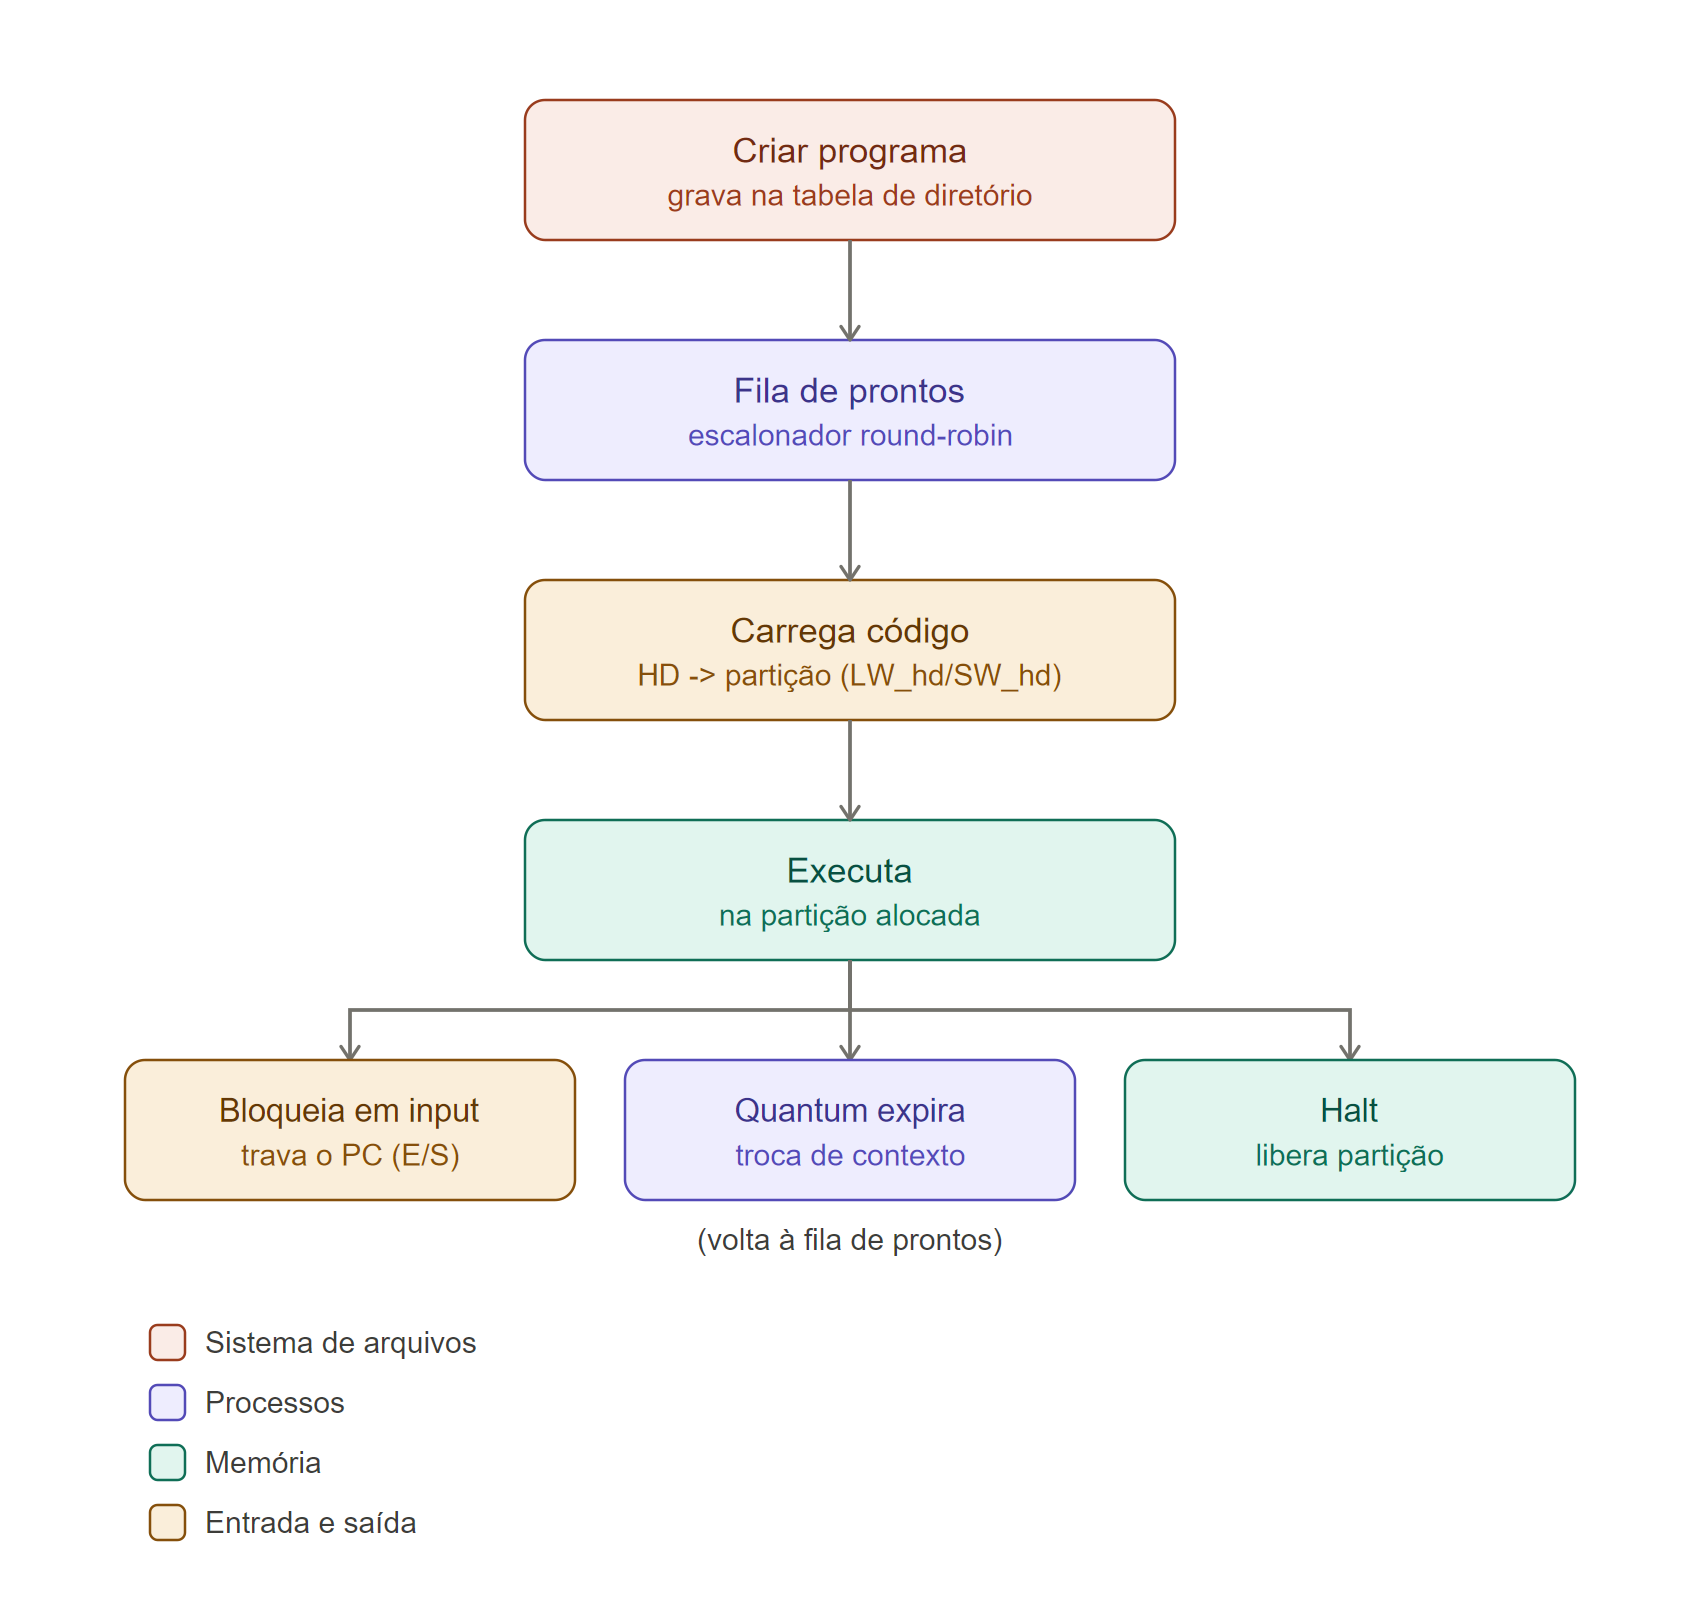
\includegraphics[width=\textwidth]{Figuras/integracao.png}
  \fonte{Autoria própria.}
\end{figure}


% ==========================================================
\chapter{Considerações Finais}
% ==========================================================

Este relatório especificou o projeto de um sistema operacional para a arquitetura
RISC-V RV32IM e o compilador da linguagem C- desenvolvidos nas etapas anteriores da
disciplina. Foram definidas as técnicas e os algoritmos para os quatro gerenciamentos
fundamentais (processos, memória, sistema de arquivos e dispositivos de E/S),
cada um apoiado em levantamento teórico e justificado diante das restrições
concretas da plataforma de hardware disponível. A Seção~\ref{sec:integracao} descreveu, de forma integrada, como esses quatro
gerenciamentos se articulam ao longo do ciclo de vida de um processo, e o
Capítulo~\ref{cap:desenvolvimento} catalogou o conjunto de alterações de
\emph{hardware} e de \emph{software}, herdadas dos laboratórios anteriores,
necessárias à execução do SO especificado.

Restam, como próximas etapas, a implementação em \emph{hardware} das alterações
especificadas (expansão e particionamento das memórias de dados e de instrução,
inclusão do temporizador e da lógica de interrupção, do HD emulado e da BIOS) e a
implementação em \emph{software} do próprio SO (o escalonador \emph{round-robin},
a rotina de troca de contexto, as operações sobre a tabela de diretório e o
\emph{shell} de comandos). A validação conjunta ocorrerá no kit FPGA DE2-115, com
os dez programas de teste definidos na etapa anterior da disciplina.

Duas dificuldades marcaram esta etapa de especificação. A primeira foi dimensionar
as partições de memória sem incorrer em suposições: como o uso de pilha de
funções recursivas depende dos valores de entrada, não havia fórmula analítica
confiável, o que exigiu simular a execução dos dez programas de teste para medir
o uso real antes de fixar o tamanho das partições. A segunda foi perceber, somente após expandir a memória de dados, que os
endereços mapeados de E/S passariam a colidir com a nova faixa de dados, um
conflito não previsto nas etapas anteriores. A solução (deslocamentos negativos,
aproveitando a extensão de sinal já existente no \emph{datapath}) exigiu
revisitar decisões que já pareciam encerradas.

\phantompart


% ----------------------------------------------------------
% ELEMENTOS PÓS-TEXTUAIS
% ----------------------------------------------------------
\postextual

% ----------------------------------------------------------
% Referências bibliográficas
% ----------------------------------------------------------
\bibliography{referencias}


% ----------------------------------------------------------
% Apêndices
% ----------------------------------------------------------

% ---
% Inicia os apêndices
% ---
\begin{apendicesenv}

% Imprime uma página indicando o início dos apêndices
\partapendices

% ----------------------------------------------------------
\chapter{BinToBCD2.v}
\label{code:BinToBCD2.v}
Código do arquivo BinToBCD2.v
\lstinputlisting{Codigos/BinToBCD2.v} 
% ----------------------------------------------------------

\end{apendicesenv}
% ---


%---------------------------------------------------------------------
% INDICE REMISSIVO
%---------------------------------------------------------------------

\phantompart

\printindex


\end{document}
